%!TEX root = ../thesis.tex

%%%%%%%%%%%%%%%%%%%%%%%%%%%%%%%%%%%%%%%%%%%%%%%%%%%%%%
%%%%%%%%%%%%%%%%%%%%%%%%%%%%%%%%%%%%%%%%%%%%%%%%%%%%%%
\subsection{Validação}
\begin{frame}{Validação}
	Três testes de validação criados
	\begin{itemize}
		\item Rede contratual simples
		\item Rede contratual com multiplas sessões
		\item Jogo de tabuleiro RISK
	\end{itemize}

	Métricas avaliadas
	\begin{itemize}
		\item Resultado da execução do teste no SAJaS e no JADE
		\item Performance em ambos os casos
	\end{itemize}
\end{frame}

\subsection{}
\begin{frame}{Validação}
	Rede Contratual Simples

	\begin{figure}
		\centering
		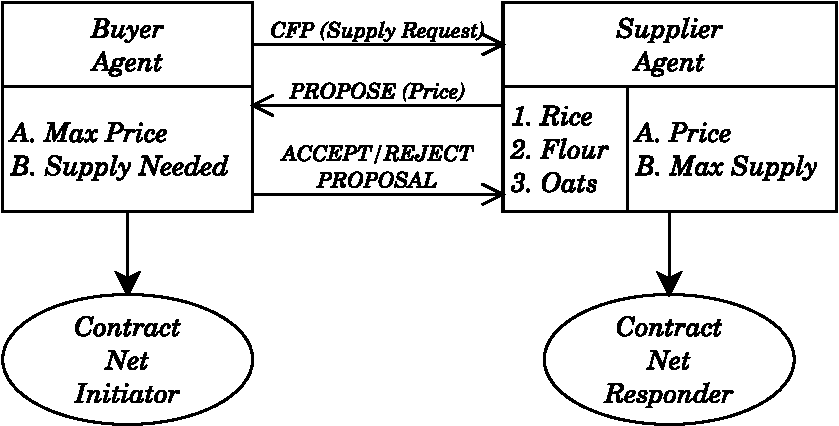
\includegraphics[height=2.3cm]{../figures/CNetExample.pdf}
	\end{figure}

	\begin{figure}
		\centering
		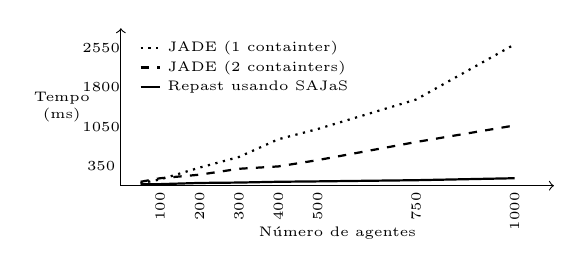
\begin{tikzpicture}[scale=0.50]
			\tiny
			% horizontal axis
			\draw[->] (0,0) -- (11,0);
			\draw (5.5,-1.2) node[align=center] {Número de agentes}; %label

			
			% labels
			\draw	%(0.5,0) node[rotate=90, anchor=east] {50}
					(1.0,0) node[rotate=90, anchor=east] {100}
					(2.0,0) node[rotate=90, anchor=east] {200}
					(3.0,0) node[rotate=90, anchor=east] {300}
					(4.0,0) node[rotate=90, anchor=east] {400}
					(5.0,0) node[rotate=90, anchor=east] {500}
					(7.5,0) node[rotate=90, anchor=east] {750}
					(10.,0) node[rotate=90, anchor=east] {1000};

			\draw	(-0.5,0.5) node[anchor=center] {350}
					(-0.5,1.5) node[anchor=center] {1050}
					(-0.5,2.5) node[anchor=center] {1800}
					(-0.5,3.5) node[anchor=center] {2550};
			% vertical axis
			\draw[->] (0,0) -- (0,4);
			\draw (-1.5,2) node[align=center] {Tempo\\(ms)}; %label
			%\draw (-1.5,1.6) node[align=center] {(ms)}; %label

			%% Data %%
			% JADE 2 containers
			\draw[thick,dashed] (0.5,3.0) --
				(1,3.0) node[anchor=west, pos=1.0] {JADE (2 containters)}; %subtitle
			\draw[thick,dashed] (0.5, 0.10) --
						(1.0, 0.19) --
						(2.0, 0.28) --
						(3.0, 0.43) --
						(4.0, 0.49) --
						(5.0, 0.65) --
						(7.5, 1.11) --
						(10., 1.53);
			% JADE 1 containers
			\draw[thick,dotted] (0.5,3.5) --
				(1,3.5) node[anchor=west, pos=1.0] {JADE (1 containter)}; %subtitle
			\draw[thick,dotted] (0.5, 0.06) --
						(1.0, 0.16) --
						(2.0, 0.46) --
						(3.0, 0.73) --
						(4.0, 1.18) --
						(5.0, 1.44) --
						(7.5, 2.19) --
						(10., 3.59);
			% Repast
			\draw[thick] (0.5,2.5) --
				(1,2.5) node[anchor=west, pos=1.0] {Repast usando SAJaS}; %subtitle
			\draw[thick] (0.5, 0.04) --
						(1.0, 0.04) --
						(2.0, 0.07) --
						(3.0, 0.08) --
						(4.0, 0.10) --
						(5.0, 0.11) --
						(7.5, 0.14) --
						(10., 0.19);
		\end{tikzpicture}
	\end{figure}
\end{frame}

\subsection{}
\begin{frame}{Validação}
	Rede contratual com múltiplas sessões. Gráficos: sucesso médio em 5 execuções ao longo 2000 contratos no SAJaS (cima) e no JADE (baixo)
	\vspace{-0.5cm}
	\begin{figure}
		\centering
		\begin{subfigure}[b]{\textwidth}
			\centering
			\begin{tikzpicture}[scale=0.4]
				\tiny

				% horizontal axis
				\draw[->] (0,0) -- (11,0);
				\draw (5.5,-1.2) node[align=center] {Número de Contratos}; %label

				% labels
				\draw	(0  ,0) node[anchor=north] {0}
						(2.5,0) node[anchor=north] {500}
						(5  ,0) node[anchor=north] {1000}
						(7.5,0) node[anchor=north] {1500}
						(10 ,0) node[anchor=north] {2000};
				
				
				% vertical axis
				\draw[->] (0,0) -- (0,5);
				\draw (-1.1,2.5) node[rotate=90, anchor=south, align=center]
					{\% de sucesso}; %label
				\draw	(0, 1) node[anchor=east] {0.25}
						(0, 2) node[anchor=east] {0.50}
						(0, 3) node[anchor=east] {0.75}
						(0, 4) node[anchor=east] {1.00};
				
				

				%% Data %%

				%subtitles
				\draw[thick] (0.5,3.5) --
					(1,3.5) node[anchor=west, pos=1.0] {Usando confiança};
				\draw[thick, dotted]
					(0.5,4.5) --
					(1,4.5) node[anchor=west, pos=1.0] {Usando apenas o preço}; 

				%lines
				\input{../chapters/charts/enterprise_values_jade}


			\end{tikzpicture}
		\end{subfigure}
		\vspace{0.1cm}\\
		\begin{subfigure}[b]{\textwidth}
			\centering
			\begin{tikzpicture}[scale=0.4]
				\tiny

				% horizontal axis
				\draw[->] (0,0) -- (11,0);
				\draw (5.5,-1.2) node[align=center] {Número de contratos}; %label

				% labels
				\draw	(0  ,0) node[anchor=north] {0}
						(2.5,0) node[anchor=north] {500}
						(5  ,0) node[anchor=north] {1000}
						(7.5,0) node[anchor=north] {1500}
						(10 ,0) node[anchor=north] {2000};
				
				
				% vertical axis
				\draw[->] (0,0) -- (0,5);
				\draw (-1.1,2.5) node[rotate=90, anchor=south, align=center]
					{\% de sucesso}; %label
				\draw	(0, 1) node[anchor=east] {0.25}
						(0, 2) node[anchor=east] {0.50}
						(0, 3) node[anchor=east] {0.75}
						(0, 4) node[anchor=east] {1.00};

				%% Data %%

				%subtitles
				\draw[thick] (0.5,3.5) --
					(1,3.5) node[anchor=west, pos=1.0] {Usando trust};
				\draw[thick, dotted] 
					(0.5,4.5) --
					(1,4.5) node[anchor=west, pos=1.0] {Usando apenas o preço}; 
				
				%lines
				\input{../chapters/charts/enterprise_values_sajas}


			\end{tikzpicture}
		\end{subfigure}
	\end{figure}
\end{frame}

\subsection{}
\begin{frame}{Validação}
	Jogo de tabuleiro RISK. Gráfico: performance de um jogo de Risk com 5 agentes durante 8 segundos.
	\begin{figure}
		\begin{subfigure}[b]{0.5\textwidth}
			\begin{tikzpicture}[scale=0.40]
			\tiny
				% horizontal axis
				\draw[->] (0,0) -- (11,0);
				\draw (5.5,-1.2) node[align=center] {Tempo/s}; %label

				% labels
				\draw	(1.25,0) node[anchor=north] {1}
						(2.5,0)	 node[anchor=north] {2}
						(3.75,0) node[anchor=north] {3}
						(5,0)	 node[anchor=north] {4}
						(6.25,0) node[anchor=north] {5}
						(7.5,0)	 node[anchor=north] {6}
						(8.75,0) node[anchor=north] {7}
						(10,0)	 node[anchor=north] {8};
				
				% vertical axis
				\draw[->] (0,0) -- (0,5);
				\draw (-1.1,2.5) node[rotate=90, anchor=south, align=center]
					{Número de rondas}; %label
				\draw	(0, 1) node[anchor=east] {30}
						(0, 2) node[anchor=east] {60}
						(0, 3) node[anchor=east] {90}
						(0, 4) node[anchor=east] {120};

				%% Data %%

				%subtitle
				\draw[thick,thick] (0.5,3.5) --
					(1,3.5) node[anchor=west, pos=1.0] {SAJaS};
				%line
				\draw[thick, dotted]%subtitle
					(0.5,4.5) --
					(1,4.5) node[anchor=west, pos=1.0] {JADE}; 
				\input{../chapters/charts/risk_times}

			\end{tikzpicture}
		\end{subfigure}
		\begin{subfigure}[b]{0.5\textwidth}
			\centering
			\includegraphics[height=3cm]{../figures/risk_GUI.png}
		\end{subfigure}
	\end{figure}
\end{frame}
